\chapter{Eigene Implementierung}
\label{sct:implementation}

\section{Kompilierung}

%Versucht man mit \lstinline!Rootbeer.jar! eine jar-Datei, welche auch Scala-Klassen beinhaltet, in GPU-Code umsetzen zu lassen, z.B. auf diese Weise:
%
%\begin{lstlisting}[language=bash]
%scalac $< -classpath $(ROOTBEER_ROOT)/Rootbeer.jar:. -deprecation
%javac $< -classpath $(ROOTBEER_ROOT)/Rootbeer.jar:.
%scalac $< -classpath $(ROOTBEER_ROOT)/Rootbeer.jar:. -deprecation
%jar -cvfm MontePiGPU.jar.tmp.jar manifest.txt *.class
%java -jar Rootbeer.jar MontePiGPU.jar.tmp.jar MontePiGPU.jar -64bit -computecapability=sm_30
%\end{lstlisting}
%
%Dann kommt es bei soot zu einer Runtime Exception:
%
%\begin{lstlisting}
%java.lang.RuntimeException: cannot get resident body for phantom class : <MonteCarloPiKernel$$anonfun$gpuMethod$1: void <init>(MonteCarloPiKernel,scala.runtime.ObjectRef)>; maybe you want to call c.setApplicationClass() on this class!
%	at soot.SootMethod.retrieveActiveBody(SootMethod.java:316)
%	at soot.rbclassload.RootbeerClassLoader.loadScene(RootbeerClassLoader.java:857)
%	at soot.rbclassload.RootbeerClassLoader.loadNecessaryClasses(RootbeerClassLoader.java:320)
%	at org.trifort.rootbeer.entry.RootbeerCompiler.setupSoot(RootbeerCompiler.java:198)
%	at org.trifort.rootbeer.entry.RootbeerCompiler.compile(RootbeerCompiler.java:219)
%	at org.trifort.rootbeer.entry.RootbeerCompiler.compile(RootbeerCompiler.java:213)
%	at org.trifort.rootbeer.entry.Main.run(Main.java:208)
%	at org.trifort.rootbeer.entry.Main.main(Main.java:244)
%\end{lstlisting}
%
%"Phantom classes are implicitly created models of classes that do not exist on Soot's classpath. To get rid of this problem, make sure that the class you are referencing is on Soot's classpath." \url{http://stackoverflow.com/questions/27383832/why-is-soot-always-saying-that-the-class-i-want-to-load-is-a-phantom-class-even}
%
%Nachdem nun also \lstinline!spark-library.jar! hinzugefügt wurde, verschwindet diese exception, aber Rootbeer findet die Kernel-Implementierung nicht:
%\begin{lstlisting}
%There are no kernel classes. Please implement the following interface to use rootbeer:
%org.trifort.runtime.Kernel
%\end{lstlisting}
%
%Dies könnte daran liegen, das \lstinline!MonteCarloPiKernel.scala! scala benutzt. Dadurch wird für \texttt{soot} verschleiert, dass die Klasse \texttt{Kernel} implementiert.
%Eine Implementierung in java löst das Problem jedoch nicht. Vermutlich weil \texttt{soot} oder \texttt{Rootbeer} nur Klassen analysieren die von der main-Klasse aufgerufen werden. Da die  main-Klasse aber in scala geschrieben ist, ist der Aufruf womöglich für \texttt{soot} nicht sichtbar, sodass \texttt{soot} \texttt{MonteCarloPiKernel.class} als unbenutzt einstuft und ignoriert. Ein Hinweis darauf liefert diese Ausgabe von Soot bei der Ausführung von Rootbeer:
%\begin{lstlisting}
%Total loaded classes: 557
%Total loaded methods: 0
%\end{lstlisting}
%Bei der Java-Version funktioniert die Kompilierung mit Rootbeer und die Ausgabe ist:
%\begin{lstlisting}
%Total loaded classes: 1428
%Total loaded methods: 4385
%\end{lstlisting}
%Eine mögliche Lösung wäre es eine Dummy-Java-Klasse zu schreiben die alle Kernel-Implementierungen aufruft und als main-class im Manifest festgelegt ist.
%Das Problem hierbei ist jedoch, dass Rootbeer Serialisierungs- und Deserialisierungscode in die aufrufende Klasse injeziert. Damit dieser injezierte Code also nicht in die Dummy-Klasse eingesetzt wird, braucht es noch eine Wrapper-Klasse, welche die Kernel-Implementierung aufruft und von der Dummy-Klasse aufgerufen wird. Dies ist \texttt{MonteCarloPi.java}.
%
%Nachdem die Kompilierung mit \texttt{Rootbeer} dann erfolgt ist, muss die Manifest-Datei \texttt{META-INF/MANIFEST.MF} dann nur noch abgeändert werden, damit sie nicht mehr auf die Dummy-Klasse verweist. Durchgeführt wurde es ähnlich, jedoch wurden alle nicht für Rootbeer relevanten Klassen erst nach dem Rootbeer-Aufruf zusammen mit der neuen Manifest-Datei in eine jar-Datei zusammengeführt, siehe Abb.\ref{fig:compilation}.


\begin{figure}[H]
	\centering
	\begin{minipage}{\linewidth}
		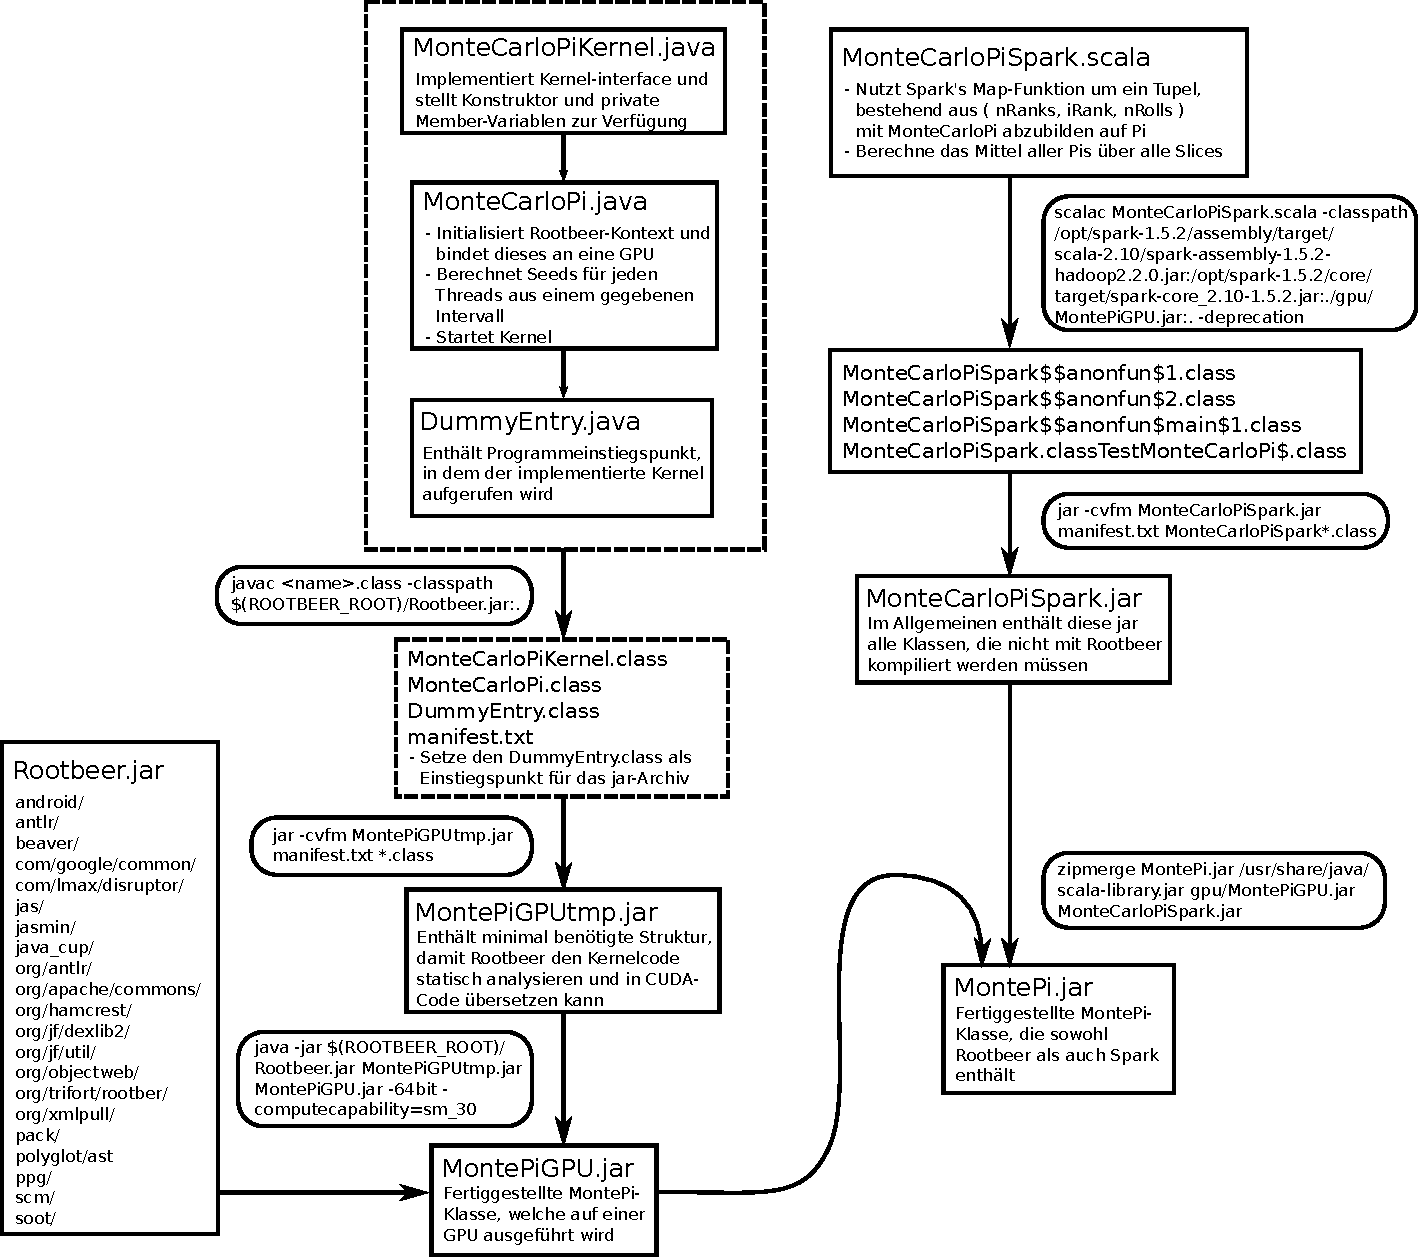
\includegraphics[width=\linewidth]{compile-structure-deu.pdf}
	\end{minipage}
	\caption{Kompilationsschema mit Kommadozeilenbefehlen und Zwischenstati.}
	\label{fig:compilation}
\end{figure}

!!! Problem: Hab mehrere Fehler gefunden deren Kenntnis möglicherweise eine Vereinfachung des Schemas bedeutet. Da bin ich noch am rumspielen, daher ist das halbfertig.

\section{Probleme}
Implementierung:
    Was ist bei GPUs zu beachten ( Seeds, 64-Bit )
    Was ist bei Rootbeer zu beachten?
      - private Variablen werden wirklich immer per memcpy hin und her transportiert.
      - muss nicht auf ungerade Kernel-Zahl achten, werden automatisch aussortiert
